\begin{refsection}[operations/minami/group.bib]
\nocite{*}
\chapter{Software Development Team}

\section{Members}

\begin{itemize}
  \item[] Kazuo Minami (Team Head)
  \item[] Masaaki Terai (Research $\&$ Development Scientist)
  \item[] Akiyoshi Kuroda (Research $\&$ Development Scientist)
  \item[] Hitoshi Murai (Research $\&$ Development Scientist)
  \item[] Kiyoshi Kumahata (Research $\&$ Development Scientist)
  \item[] Kengo Miyamoto (Research $\&$ Development Scientist)
  \item[] Yoshito Kitazawa (Research $\&$ Development Scientist)
\end{itemize}

\section{Research Activities}

Collaboration between the K computer system and its applications is key to creating innovative results. To maximize application and system performances and usability, the Software Development Team is conducting the following activities: (1) efforts to maintain the stable operation of the K computer and the support for users to obtain good outcome; (2) research into the high level operational efficiency of the K computer; and (3) research to improve application performances.

\section{Research Results and Achievements}

%Text for research Results and achievements. Journal-artcile~\cite{sample-journal}.
%Conference-paper~\cite{sample-conference}.
%Invited-talk~\cite{sample-invited}.

\subsection{Operations of the K Computer}
\subsubsection{Improvement of the Operation Environment}
\begin{enumerate}
\renewcommand{\labelenumi}{(\arabic{enumi})}

\item Establish the rules for installing and maintaining open source software (OSS)

The installed software requires continuous maintenance because software compiled in an older language environment of the K computer may have trouble in the current newer language environment owing to discrepancies between the compiling and running environments.

Formerly, the maintenance rules for installed software were not sufficiently established. Therefore, we needed to judge whether maintenance for previously installed software was necessary when a trouble occurred. In FY2015, to improve usability, we established overall rules concerning OSS management.

\item Study on runtime fluctuations

Runtime fluctuations are differences in the runtime of an application that occur for some reason on the system despite the application being carried out under the same execution conditions and in the same manner. These fluctuations disturb efficient operations on the K computer. Therefore, we need to study runtime fluctuations and resolve them.

In FY2015, we encountered an application with a runtime fluctuation. A detailed analysis, e.g., using a profiler, special compile options, and monitoring values in the calculation, found an increased number of executed instructions and irregular floating point values when the runtime increased.

This irregular floating point value is called the ``de-normalized number'' and is defined in IEEE754. Usually, floating point calculations should be executed by the hardware; however, in this case, the calculation of the de-normalized number was carried out by the software. Therefore, an increased number of instructions were executed and more time was consumed when the de-normalized number was included in a program. We confirmed this phenomenon using a simple test program. Currently, we are investigating whether this is the actual cause of the runtime fluctuation in the application.

\item Checking the system performance

 When system software, such as operating systems, compilers, and libraries, are updated, we need to check if the update has any side effects on the execution of the applications. Therefore, we regularly test the performance. In FY2015, we had two consecutive updates of the language environments, K-1.2.0-18 and K-1.2.0-19, and we checked each environment using the check suite, which is a tool to check the comprehensive system performance.

 \begin{enumerate}
  \renewcommand{\labelenumii}{\arabic{enumii})}
  \item K-1.2.0-18
   \begin{itemize}
    \renewcommand{\labelitemi}{-}
    \item According to the result of the check suite, we detected performance degradations.
    \item As a result of an investigation, we determined that the cause of the degradations was not the language environment, which included the compilers and the libraries. Therefore, K-1.2.0-18 was formally released to all users.
   \end{itemize}
  \item K-1.2.0-19
   \begin{itemize}
    \renewcommand{\labelitemi}{-}
    \item According to the result of the check suite, the performance was the same as the old environment. It was then formally released to all users.
   \end{itemize}
 \end{enumerate}

\item Release of the MPI performance data

 In FY2015, we checked the performance of the major communication functions in the MPI library, measured in FY2014, and released it as a tutorial to all users as a reference to the communication performance. We researched trends in the performance using the Tofu specific algorithm, message size, node shape, and environment variables. Using the results, we described the trends in the performance in the tutorial. Further, we provided the data of the measured results~\cite{MPI_HPC}.

\item Evaluation of the FX100 System

 We compared the performance of the K computer and FX100 via a collaboration with RIKEN ACCC. Using the check tool for the K computer, we evaluated the calculation and communication performances. Because the communication performance of the inner node was lower than that of the outer node, there were cases where the performance of the collective communication was low~\cite{HOKUSAI_FX100}.

\end{enumerate}

\subsubsection{Development of Tools}
\begin{enumerate}
\renewcommand{\labelenumi}{(\arabic{enumi})}

\item K-scope: The Fortran and C source code analysis tool

K-scope is a Fortran and C source code analysis tool that uses intermediate codes exported by the front-end of the Omni compiler. To find bottlenecks (e.g., multiple nested loops) from source codes, performance engineers can use K-scope prior to rewriting source codes to improve performance. In FY2015, to improve the usability of the tool, we extended the keyword search feature in the C version of the tool. In addition, we developed a feature that extracts a kernel code (a tiny program including a few subroutines or loops to quickly evaluate performance) from Fortran source codes. We have distributed K-scope since FY2012 as part of the AICS software. Furthermore, in collaboration with Kobe University in Japan, we developed the Eclipse plugin to visualize Fortran source code structure on the framework.

\item Creating simple methods to analyze application performance

 SPARC64 VIIIfx has more than 100 hardware counters for performance measurement. To collect detailed profiling data of an application, it was previously necessary to execute the profiler several times. In FY2015, we developed simple profile tools that are each executed once. These tools are the basic performance analysis and the time breakdown analysis. Using these tools, the user can collect profiling data by executing the profiler once. We will release the tools to users.

\end{enumerate}

\subsubsection{User Support}

We provide user support services from the K support desk in collaboration with the system operations and development team. The K support desk's role is to solve any queries from the users, which come from both RIKEN AICS users and general users indirectly via the Research Organization for Information Science and Technology (RIST). RIST is an official organization that is engaged in consultation services for the K computer general users. We are in charge of compilers, profilers, programming support tools, debuggers, numerical libraries, an MPI library, user manuals, and tutorial documents.

The K support desk accepted 756 technical inquiries, requests, and problem reports in FY2015. The staff members of the K support desk held weekly meetings to check the progress towards solving these issues.

\subsection{ Improvement of the operational efficiency and power consumption reduction}
 The effective use of computing resources for the operation of the K computer is important. Improving the job performance to improve the operational efficiency and to reduce the power consumption is necessary. Here, operational efficiency improvement means saving computational resources. We constructed a system to collect information concerning jobs and to analyze the jobs to improve their operational efficiency.
 
\subsubsection{Development of a collection system for the job information}

A comprehensive statistical analysis to improve the operational efficiency is difficult because massive amounts of job information (e.g., flops, memory throughput, and I/O etc.) are separately managed in several different servers. In FY2015, to gather the statistical information from the separate databases, we performed a feasibility study and constructed a proto-system. This system transparently collects the information and does not require additional tasks (e.g., profilers) for the users. We estimate that the constructed database will reach 1GB in a year. Furthermore, the database will continue to expand with the incorporation of additional information. Moreover, we developed a set of tools for job analyses to efficiently analyze these big data. Using the system, we will publish this information to users via a portal site.

\subsubsection{Analysis of job information}

\begin{figure}[p]
\centering
  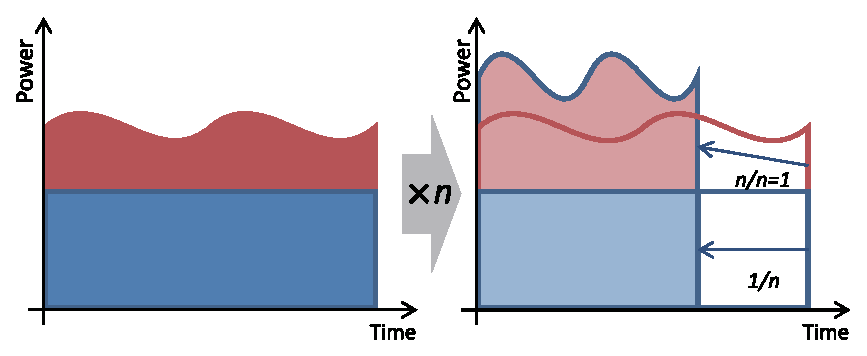
\includegraphics[width=0.5\textwidth,keepaspectratio,width=10cm]
  {operations/minami/Fig-3-1.eps}
  \caption{ Relation between power consumption and application performance. The blue region indicates standby power and the red region is the power that is proportional to the performance.}
  \locallabel{fig:operatons-minami-Fig-3-1}

\vspace{1.5cm}

\centering
  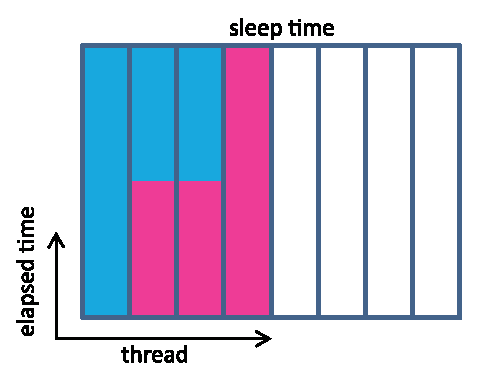
\includegraphics[width=0.5\textwidth,keepaspectratio,width=5cm]
  {operations/minami/Fig-3-2.eps}
  \caption{ The concept of sleep time. The blue region is the CPU working time, the purple region is the waiting time caused by communication and imbalance, and the white region is the time spent not running. We took the sum of the purple and white regions to be the sleep time.}
  \locallabel{fig:operatons-minami-Fig-3-2}

\vspace{1.5cm}

\centering
  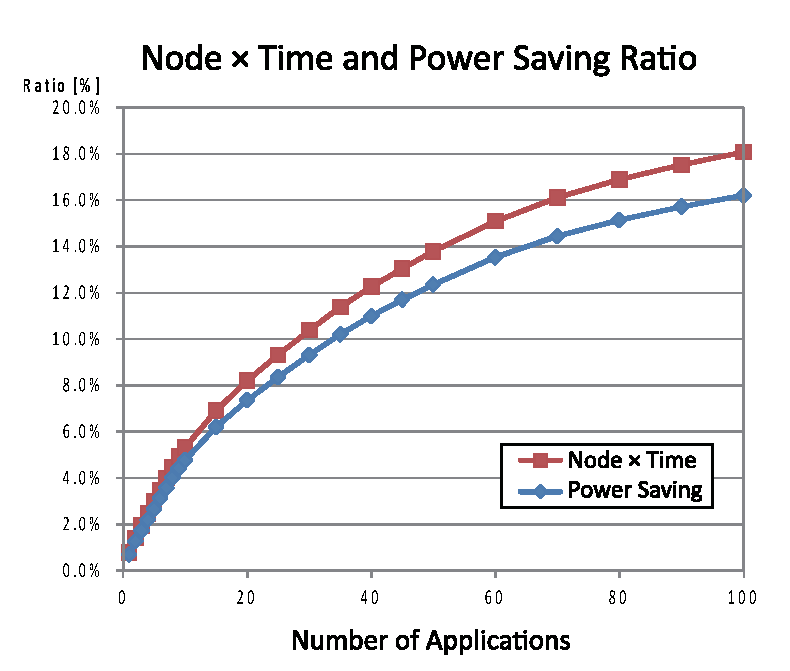
\includegraphics[width=0.5\textwidth,keepaspectratio,width=8cm]
  {operations/minami/Fig-3-3.eps}
  \caption{ Relation between the number of evaluation applications and the calculated savings in resources and power consumption reduction.}
  \locallabel{fig:operatons-minami-Fig-3-3}
\end{figure}

To improve the operational efficiency of the K computer, we analyzed the statistical information extracted from the database. Via the analysis, we expect to find problems in terms of improving operations. In addition, based on the profiling data, we can illustrate the relation between the application performance and power consumption~\cite{POWER_ACS}~\cite{POWER_AICS}~\cite{POWER_AXIES}. In FY2015, we determined the dominant power consumption factors on the K computer. One of the factors is the standby power consumption, which is a constant wastage regardless of whether an application is running. In other words, the power consumption is a two-storied structure: a basic part (standby power) and an increments part (active power). Therefore, a reduction in the execution time via performance improvement will contribute to saving computational resources. Even though the power consumption per second is increased by application tuning, the total power consumption will be reduced by decreasing the dominant standby power, as shown in Fig.~\localref{fig:operatons-minami-Fig-3-1}.

Therefore, to improve the operational efficiency and reduce the power consumption, we plan to measure the actual application performance including the production runs and improve them based on the following metrics: 1) memory performance, 2) calculation performance, 3) I/O performance, and 4) communication performance. In particular, the memory and calculation performances are major factors in power consumption. These factors can be analyzed from the hardware counter information. In addition, we found that the I/O performance has an imbalance. The amount of communication traffic was evaluated using a function of the operating system. However, the communication time is difficult to analyze because it is not constructed from the collected data. Therefore, to address this problem, we introduced sleep time, which includes the communication and waiting time due to the imbalance of the calculations (Fig.~\localref{fig:operatons-minami-Fig-3-2}).

A job that requires large computational resources occupies a greater proportion of the total system resources. We employed a weighted average using the compute node time product and classified the jobs into fields, such as Earth science and materials science. Using this analysis, with the average performance in each field, we estimate that a 5.3\% improvement in the operational efficiency would result from improving the top 10 major applications using computational resources on the K computer. In addition, an 8\% improvement is estimated when improving the top 20 applications~\cite{POWER_SC15} (Fig.~\localref{fig:operatons-minami-Fig-3-3}). A large usage improvement can be expected by evaluating just part of the applications. In addition, we found that the computational resources spend huge amounts time in sleep time due to communication and load imbalances in these applications.

\subsection{Research and Development of Techniques to Improve the Computational Performance of Application Programs}
\subsubsection{HPCG performance improvement on the K computer}

The high-performance conjugate gradient (HPCG) benchmark program has been proposed as a realistic performance metric for supercomputers. HPCG measures the speed at which symmetric sparse linear system equations are solved using the frequently used conjugate gradient method with a multi-grid symmetric Gauss-Seidel smoother.

We evaluated and improved the performance of HPCG on the K computer using an early version prior to its official announcement. HPCG showed good parallel scalability; however, its single CPU performance was very low. Therefore, we tuned the single CPU performance using several techniques, such as memory layout improvement and multithreading. Consequently, we obtained a speed-up of approximately 19 times. The K computer marked 0.461 PFLOPS using 82,944 nodes and ranked second on the ranking of HPCG. This rank was higher than that of the Titan supercomputer at Oak Ridge National Laboratory, which has a higher LINPACK score than the K computer.

The new version of the HPCG code was released in SC15. In this version, the method for calculating the GFLOPS value was modified. Therefore, we are now attempting to obtain a high HPCG score with this new version. In the new version, the time required for creating the problem matrix is included in the total runtime for calculating the GFLOPS value. Thus, we have shortened the time required to create the problem matrix. In addition, the effect of increasing the iteration steps for convergence due to coloring is more significant in the new version. Therefore, the running parameters we previously used are no longer suitable and we are investigating additional efficient running parameters.

\subsubsection{Support for Improving the Computational Efficiency of Full-node Application Programs}
\begin{enumerate}
\renewcommand{\labelenumi}{(\arabic{enumi})}

\item ELSES

To analyze the quantum behavior of a billion atoms in an organic polymer electronic device, we optimized a simulation code based on order-$N$ method with the full system of the K computer, in collaboration with the Hoshi laboratory at the Tottori University. The hottest kernel of the code was a four-nested loop with short iteration numbers for matrix-vector multiplication. Its performance was 1\% of the K peak performance. We tried several matrix data storing formats, e.g., CRS and ELL, and their corresponding implementations. As a result, it was found that the performance of this kernel could reach 16\% of the K peak performance.

In a performance evaluation with strong scaling on the full compute nodes, we achieved 72\% in parallel efficiency and minimized the time-to-solution (less than $10^2$ s in elapsed time) to realize practical research. Based on this achievement, we submitted a paper for the ACM Gordon Bell Prize in SC16.
 
Furthermore, the knowledge obtained in the collaboration contributed to improvements in the profiler and environment on the K computer.

\item DMRG

 This application approximately calculates the electronic states in a crystal using the density matrix renormalization group method for a strongly correlated quantum system. We supported tuning and measuring the detailed performance of this application. There are two parameters. One is the number of sites to decide the size of a system, and the other is the DMRG truncation number to decide the precision. In the ground state calculation for a 1D system, which is a model on a 16-site cluster with a truncation number of m = 8064, we achieved a peak performance of more than 70\% using all 82,944 nodes on the K computer. In addition, we calculated the dynamics in 2D, using a model on a 24$\times$18 site cluster with a truncation number of m = 4032, on the K computer.

\item PHASE

We have continually supported the first-principles density functional theory calculation application PHASE, to be developed by NIMS to apply for the ACM Gordon Bell Prize in SC15, with further tuning and measurements. This fiscal year, we further improved its performance via a parameter optimization search. The application performance improved to 21.17\% (2.25 PFLOPS) this fiscal year from 18.6\% (1.97 PFLOPS) last fiscal year. In a strong scaling measurement using approximately 4,000 atoms, whose scalability was achieved on 36,864 nodes last fiscal year, we achieved scalability to 82,944 nodes. This means that we can calculate a structural relaxation calculation problem that required 51 days using 48 nodes within 8 hours. We were able to simulate long time relaxation using a number of compute nodes that was much larger than the number of atoms.

\end{enumerate}

\subsubsection{Speeding Up a Kernel Program to Multiply a Double-double Precision Matrix by a Double Precision Vector}

We improved the computational efficiency of a one-process kernel program to multiply a double-double precision matrix by a double precision vector. The elapsed time of the kernel program was reduced to less than 1/3 on 8 cores of the K computer and 1/8 on 12 cores of an FX100 system in a case where the matrix size was 24 rows and 393,216 columns.

We stopped the unrolling of a loop of the matrix row number, which was the outermost loop, to reduce cache line conflicts by decreasing the number of data streams. We abolished the unnecessary double-double precision extension of the vector so that the thrashings resulting from prefetches on the L1D cache were reduced. For the inner product procedure contained in the row number loop, we adopted a tournament sum scheme so that the SIMD arithmetic units would effectively work.

\subsubsection{Graph-based Economic Simulation}

To study behavior in economic networks, a graph-based algorithm was proposed. The algorithm propagates financial stress in a network based on actual transactions among domestic companies. To perform massive parameter-sweep calculations, we needed to reduce the turnaround time in a graph traversal. In FY2015, based on a prototype code in C++, we developed new code in C with OpenMP. In addition, we employed a MapReduce framework to quickly deploy workloads to compute nodes on the K computer. Using the framework on the bulk-job mode, the turnaround time was reduced to 192 s from more than 9 hours (175 times faster). This research project was conducted in collaboration with University of Hyogo.

\subsubsection{Evidenced-based Performance Tuning}

Typical performance improvements for an application comprise two steps: finding a bottleneck using profilers and rewriting the source code. These steps are a form of engineering; however, the performance is strongly influenced by rewriting of the source code. Eventually, we often use an ad-hoc solution instead of engineering with sufficient investigation. Therefore, even if we have tips and know-how regarding performance optimizations for an application, it is difficult to systematically marshal this knowledge and reuse it for other similar applications. In FY2015, to perform a feasibility study to classify source code behavior with supervised learning, we collected more than 50 open source projects including more than 100 loops from GitHub to create training data from public resources. This study was conducted in collaboration with the HPC Usability Research Team in RIKEN AICS.

\section{Schedule and Future Plan}

The Software Development Team will continue the following activities in the next fiscal year:  (1) efforts concerning the stable operation of the K computer and support for users to obtain good outcomes; (2) research into the high level operational efficiency of the K computer; and (3) research to improve application performances. We will evaluate the detailed behavior of applications contributing to the improvement of the operational efficiency in cooperation with developers.

%%% DO NOT EDIT BELOW

\section{Publications}

%\printbibliography[keyword=journal, heading=subbibliography, title={Journal Articles}, prefixnumbers={1-}, resetnumbers=true]
%\printbibliography[keyword=proceedings, heading=subbibliography, title={Conference Papers}, prefixnumbers={2-}, resetnumbers=true]
%\printbibliography[keyword=invited, heading=subbibliography, title={Invited Talks}, prefixnumbers={3-}, resetnumbers=true]
%\printbibliography[keyword=poster, heading=subbibliography, title={Posters and Presentations}, prefixnumbers={4-}, resetnumbers=true]
%\printbibliography[keyword=deliverable, heading=subbibliography, title={Patents and Deliverables}, prefixnumbers={5-}, resetnumbers=true]

\printbibliography[keyword=journal, heading=subbibliography, title={Journal Articles}, resetnumbers=true]
\printbibliography[keyword=proceedings, heading=subbibliography, title={Conference Papers}]
\printbibliography[keyword=invited, heading=subbibliography, title={Invited Talks}]
\printbibliography[keyword=poster, heading=subbibliography, title={Posters and Presentations}]
\printbibliography[keyword=deliverable, heading=subbibliography, title={Patents and Deliverables}]

\end{refsection}
